\documentclass{article}
\newcommand\tab[1][1cm]{\hspace*{#1}}
\usepackage{amssymb,amsmath,graphicx,float}
\begin{document}
For the Species HCO, I compared the difference between it's Nasa 7 and Nasa 9 thermo coefficients. Since the Nasa 9 coefficients only differ from the 7 coefficients by containing two extra independent terms in it, we can convert the NASA 7 form into NASA 9 by just setting these to 0. The different equations for the $C_p$, H, and S are given as:\\
\\
\tab In Nasa 9( $a_7$ is always 0):
\begin{align*}
  \frac{C_P}{R} = \quad &a_0T^{-2} + a_1T^{-1} + a_2+a_3T + a_4T^2 + a_5T^3 + a_6T^4\\
  \frac{H}{RT} = -&a_0t^{-2} + a_1\frac{ln{T}}{T} + a_2 + a_3\frac{T}{2} + a_4\frac{T^2}{3} + a_5\frac{T^3}{4} + a_6\frac{T^4}{5} + \frac{a_8}{T}\\
  \frac{S}{R} =  -&a_0\frac{T^{-2}}{2} - a_1T^{-1} + a_2ln{T} + a_3T + a_4\frac{T^{2}}{2} + a_5\frac{T^3}{3} + a_6\frac{T^4}{4} + a_9\\
\end{align*}
\tab For Nasa 7 in the Nasa 9 format, the coefficients $a_0,a_1 = 0$. By using these equations I was able to compute$C_p$, H, and S for each of the coefficients in their respective Temperature intervals and compare them. These Figures are located below:

  \begin{figure}
  \centering
  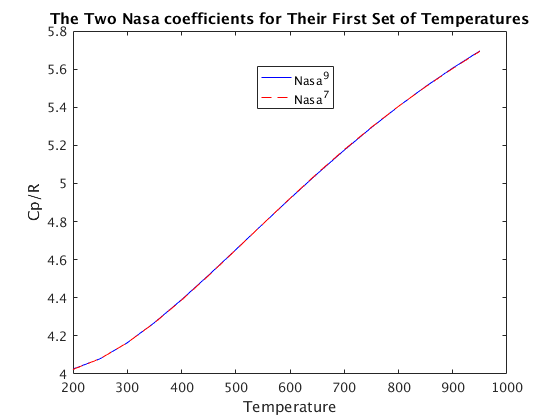
\includegraphics[width=\textwidth]{Cp1.png}
  \label{fig:cp1}
  \caption{HCO comparison of Nasa 7 vs Nasa 9 data}
\end{figure}



\begin{figure}
  \centering
  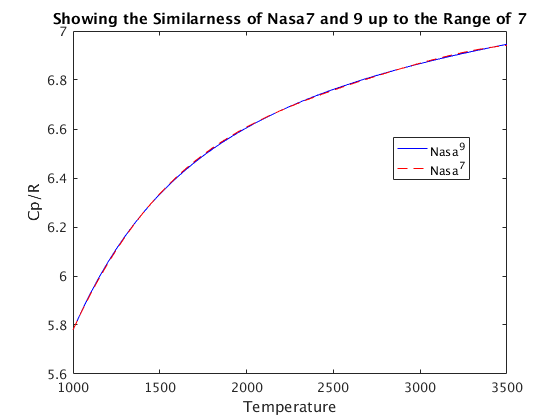
\includegraphics[width=\textwidth]{Cp2.png}
  \label{fig:cp2}
  \caption{HCO comparison of Nasa 7 vs Nasa 9 data}
\end{figure}


\begin{figure}
  \centering
  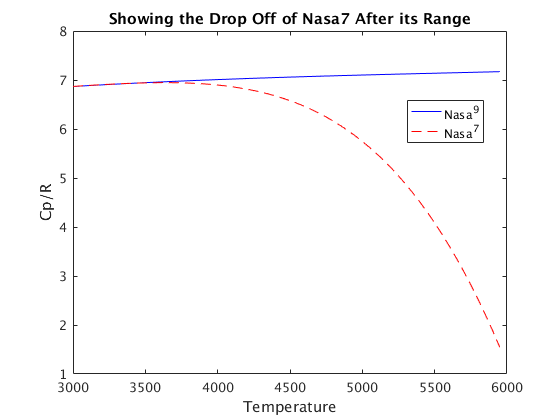
\includegraphics[width=\textwidth]{Cp3.png}
  \label{fig:cp3}
  \caption{HCO comparison of Nasa 7 vs Nasa 9 data}
\end{figure}


\begin{figure}
  \centering
  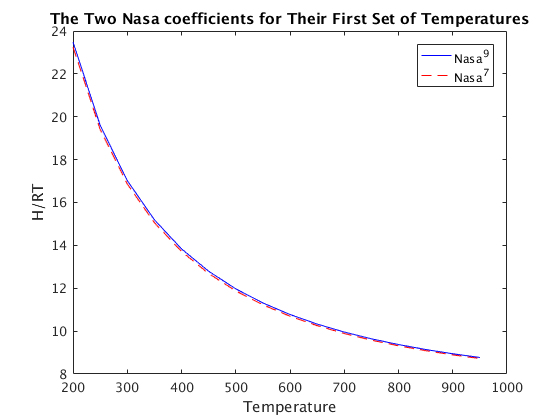
\includegraphics[width=\textwidth]{H1.png}
  \label{fig:H1}
  \caption{HCO comparison of Nasa 7 vs Nasa 9 data}
\end{figure}


\begin{figure}
  \centering
  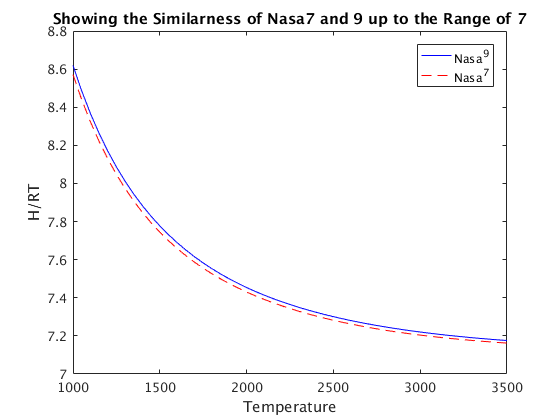
\includegraphics[width=\textwidth]{H2.png}
  \label{fig:H2}
  \caption{HCO comparison of Nasa 7 vs Nasa 9 data}
\end{figure}


\begin{figure}
  \centering
  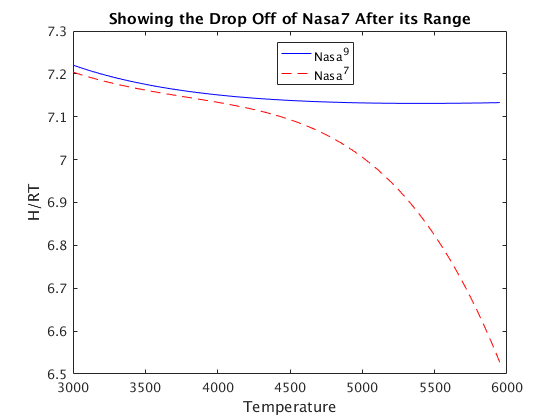
\includegraphics[width=\textwidth]{H3.png}
  \label{fig:H3}
  \caption{HCO comparison of Nasa 7 vs Nasa 9 data}
\end{figure}


\begin{figure}
  \centering
  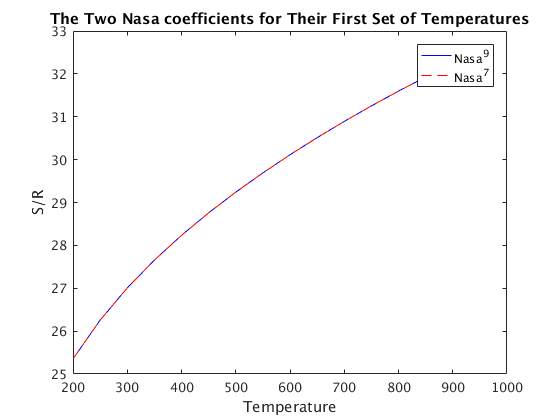
\includegraphics[width=\textwidth]{S1.png}
  \label{fig:s1}
  \caption{HCO comparison of Nasa 7 vs Nasa 9 data}
\end{figure}


\begin{figure}
  \centering
  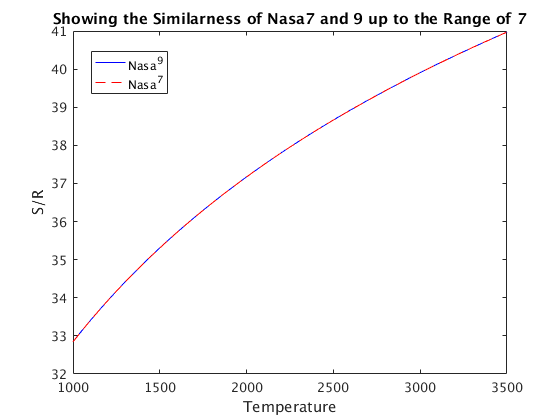
\includegraphics[width=\textwidth]{S2.png}
  \label{fig:S2}
  \caption{HCO comparison of Nasa 7 vs Nasa 9 data}
\end{figure}


\begin{figure}
  \centering
  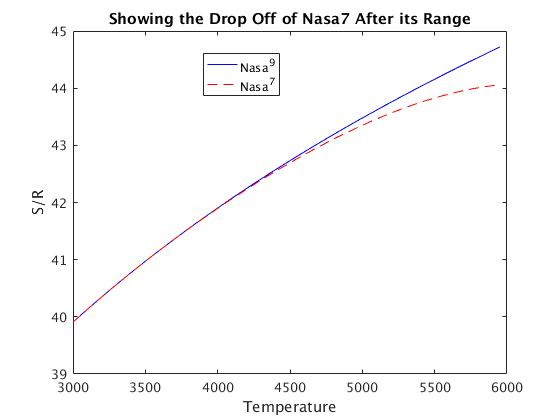
\includegraphics[width=\textwidth]{S3.png}
  \label{fig:S3}
  \caption{HCO comparison of Nasa 7 vs Nasa 9 data}
\end{figure}

\end{document}
